\documentclass[12pt, aspectratio=169]{beamer}

\usepackage{color}
\usepackage[utf8]{inputenc}
\usepackage{graphicx}
\usepackage{tikz}
\usepackage[T1]{fontenc}
\usepackage{caption}
\usepackage{wrapfig}
\usepackage{xurl}

\captionsetup[figure]{labelformat=empty}
\setbeamertemplate{section in toc}[square]

\usetheme{Singapore}
\usecolortheme{default}
\usefonttheme{structurebold}
\setbeamerfont{text}{size=\large}
\setbeamercovered{dynamic}
\setbeamertemplate{bibliography item}{\insertbiblabel}

\definecolor{ao}{rgb}{0.0, 0.0, 0.7}

%\setbeamertemplate{footline}[frame number]
\setbeamertemplate{footline}[text line]{%
  \parbox{\linewidth}{\vspace*{-8pt}\color{ao}\insertshorttitle\hspace{10px}\insertshortauthor\hfill\insertpagenumber}}

\title{System Usability Scale (SUS)}
\author[Y. Höll, F. Jäpel]{Yannik Höll \& Franz Jäpel}
\date{April 26, 2022}
% \logo{
\includegraphics[keepaspectratio=True, width=30px]{./image/logo.png}}



\beamertemplatenavigationsymbolsempty 

\begin{document}
\begin{frame}[noframenumbering, plain]
	\titlepage
\end{frame}

\begin{frame}
	\frametitle{Einteilung}
	\tableofcontents
\end{frame}

\section{Was bedeutet SUS}
\begin{frame}
	\frametitle{Was bedeutet SUS}
	\begin{columns}
		% Column 1
		\begin{column}{0.7\textwidth}
			\begin{itemize}
				\item<1> Fragebogen mit festen Fragen
				\item<1> 8 Usability, 2 Learnability
				\item<1> Punktzahl 1-5
				\item<1> Formel für Gesamtpunktzahl: 
				Sei $u_n$ Punktzahl bei Frage $n$ und $G$ Gesamtpunktzahl, dann:
				\begin{math} G=((\sum\limits_{k=1}^5(u_{2k-1})-5) + (25-\sum\limits_{k=1}^5(u_{2k}))) \cdot 2.5 $\\$ \end{math}
			\end{itemize}
		\end{column}
		% Column 2    
		\begin{column}{0.3\textwidth}
			\begin{figure}
				\centering
				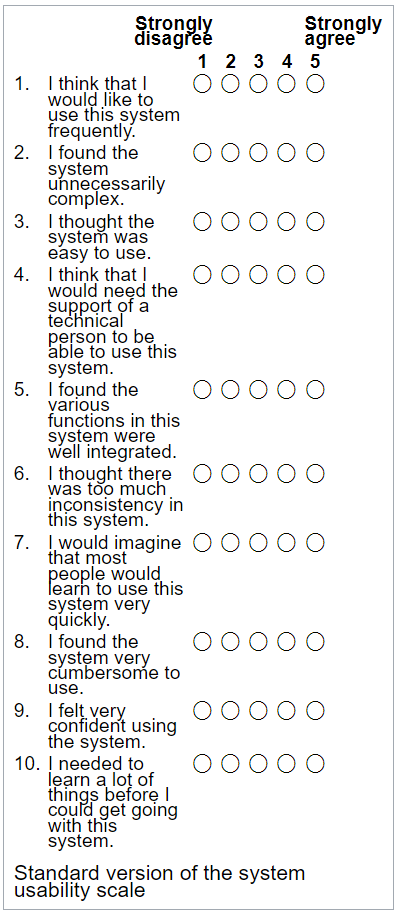
\includegraphics[keepaspectratio=true, width=65px]{./image/sus.png}
				\caption{SUS Standardfragebogen \tiny{\cite{wiki1}}}
			\end{figure}		
		\end{column}
	\end{columns}
\end{frame}

\begin{frame}
	\begin{enumerate}
		\item <1> I think that I would like to use this system frequently.
		\item <1> I found the system unnecessarily complex.
		\item <1> I thought the system was easy to use.
		\item <1> I think that I would need the support of a technical person to be able to use this system.
		\item <1> I found the various functions in this system were well integrated.
		\item <1> I thought there was too much inconsistency in this system.
		\item <1> I would imagine that most people would learn to use this system very quickly.
		\item <1> I found the system very cumbersome to use.
		\item <1> I felt very confident using the system.
		\item <1> I needed to learn a lot of things before I could get going with this system.
	\end{enumerate}
\end{frame}

\begin{frame}
	\vspace*{20px}
	\begin{itemize}
		\item <1> Verschiedene Skalen zur Interpretation SUS-Score:
	\end{itemize}
	\begin{figure}
		\centering
		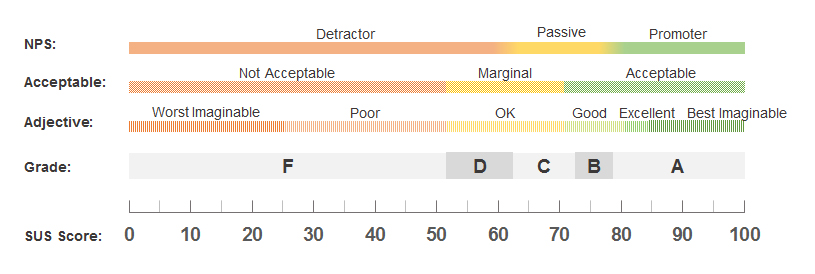
\includegraphics[keepaspectratio=true, width=\textwidth]{./image/sus-scale-adj.jpg}
		\caption{Skalen im Vergleich\tiny{\cite{pic3}}}
	\end{figure}
\end{frame}


\section{Einsatzgebiete}
\begin{frame}
	\frametitle{Einsatzgebiete}
	\begin{itemize}
		\item<1> Wenig Zeit oder finanzielle Mittel
		\item<1> In Kombination mit anderen Tests
		\item<1> Meist mit konkreter Aufgabe (test-then-measure)
		\item<1> Nicht für Erkennung genauer Probleme
	\end{itemize}
\end{frame}

	
\begin{frame}
	\frametitle{Use Cases}
	\vspace{20px}
	\begin{itemize}
		\item<1> Allgemeiner Vergleich mit ähnlichen Produkten
		\item<1> Interface-Typen/Website-Versionen vergleichen
		\item<1> Continuous Testing
	\end{itemize}
	\vspace{15px}
	\begin{figure}
		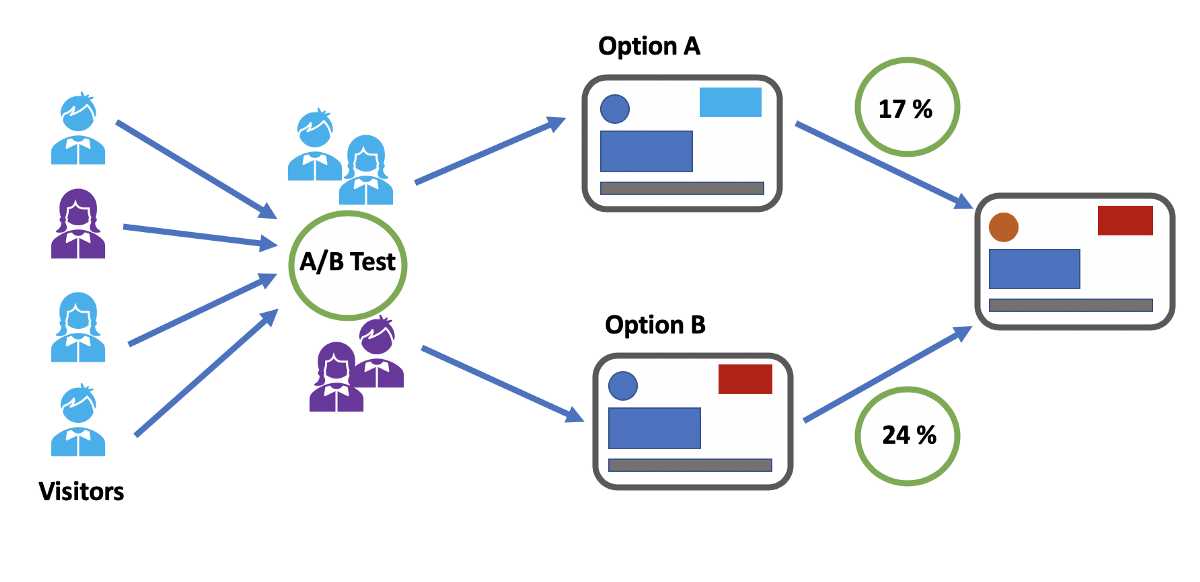
\includegraphics[keepaspectratio=true, width=200px]{./image/ab.png}
		\caption{A-B-Test \tiny{\cite{pic2}}}
	\end{figure}
\end{frame}

\section{Testablauf}
\begin{frame}
	\frametitle{Testablauf}
	\begin{columns}
		% Column 1
		\begin{column}{0.7\textwidth}
			\begin{enumerate}
				\item<1> Tester nutzt das System mit konkreter Aufgabe
				\item<1> Tester erhält den Fragebogen
				\item<1> Statistische Aufarbeitung der Ergebnisse
				\item<1> Vergleich mit anderen/ähnlichen Systemen
			\end{enumerate}
		\end{column}
		% Column 2    
		\begin{column}{0.3\textwidth}
			\begin{figure}
				\centering
				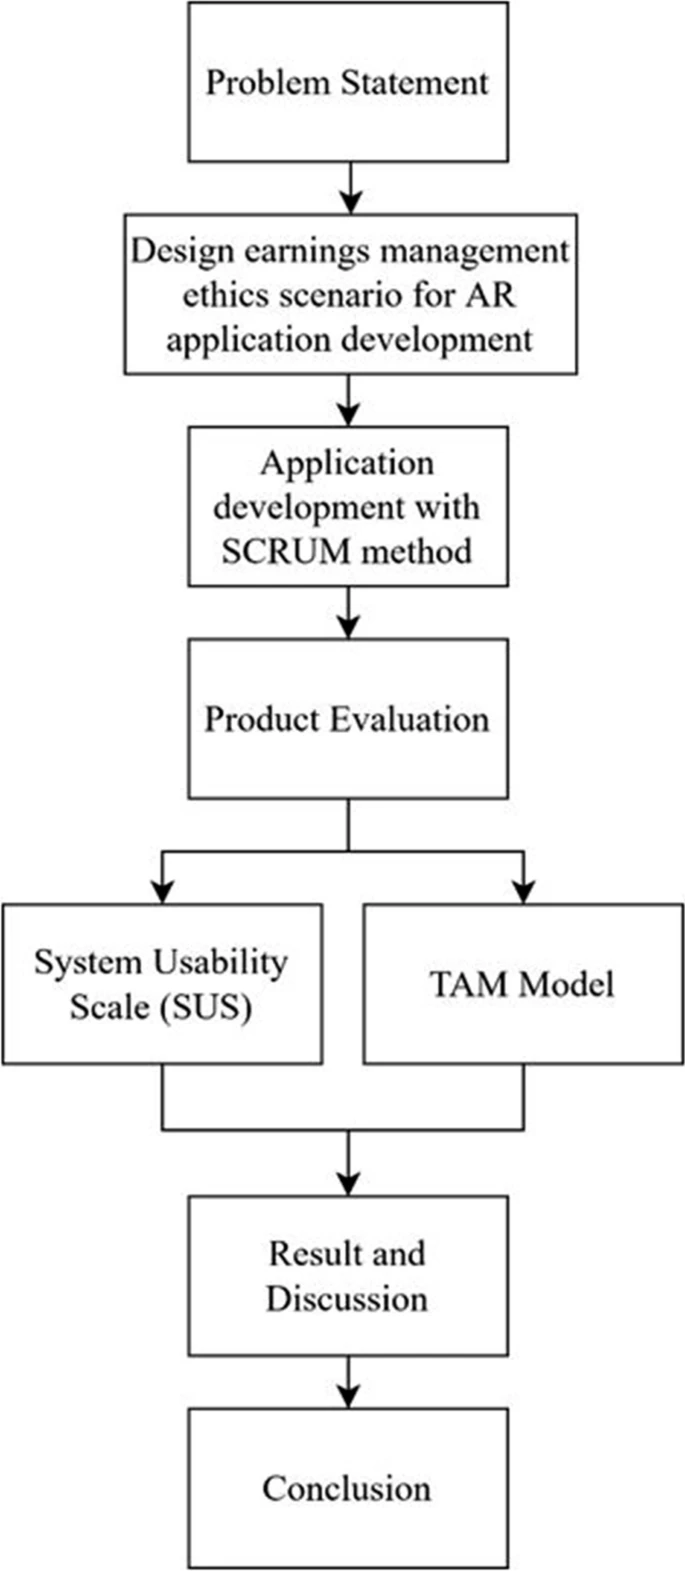
\includegraphics[keepaspectratio=true, width=75px]{./image/ablauf.png}
				\caption{Beispielablauf \tiny{\cite{young2009cultivating}}}
			\end{figure}		
		\end{column}
	\end{columns}
\end{frame}

\section{Vor- \& Nachteile}
\begin{frame}
	\frametitle{Vorteile}
	\begin{itemize}
		\item<1> Einfach vergleichbare Daten, gut für Statistik
		\item<1> Geringer Zeitaufwand
		\item<1> Gibt es schon seit 1993
		\item<1> Zeitliche Trends erkennbar
		\item<1> Selbsterklärend
		\item<1> Keine Beobachtung während des Tests nötig
		\item<1> Programmunabhängig
	\end{itemize}
\end{frame}

\begin{frame}
	\frametitle{Nachteile}
	\begin{itemize}
		\item<1> Gründe für schlechten Score nicht vorhanden
		\item<1> Vergleich zwischen Systemen nur qualitativ
		\item<1> Geringe Korrelation Effektivität - Usability
		\item<1> Vergleichbarkeit mit Test in anderen Sprachen nicht klar
	\end{itemize}
\end{frame}

\section{Beispiel}
\begin{frame}
	\frametitle{Beispiel}
		\begin{figure}
			\centering
			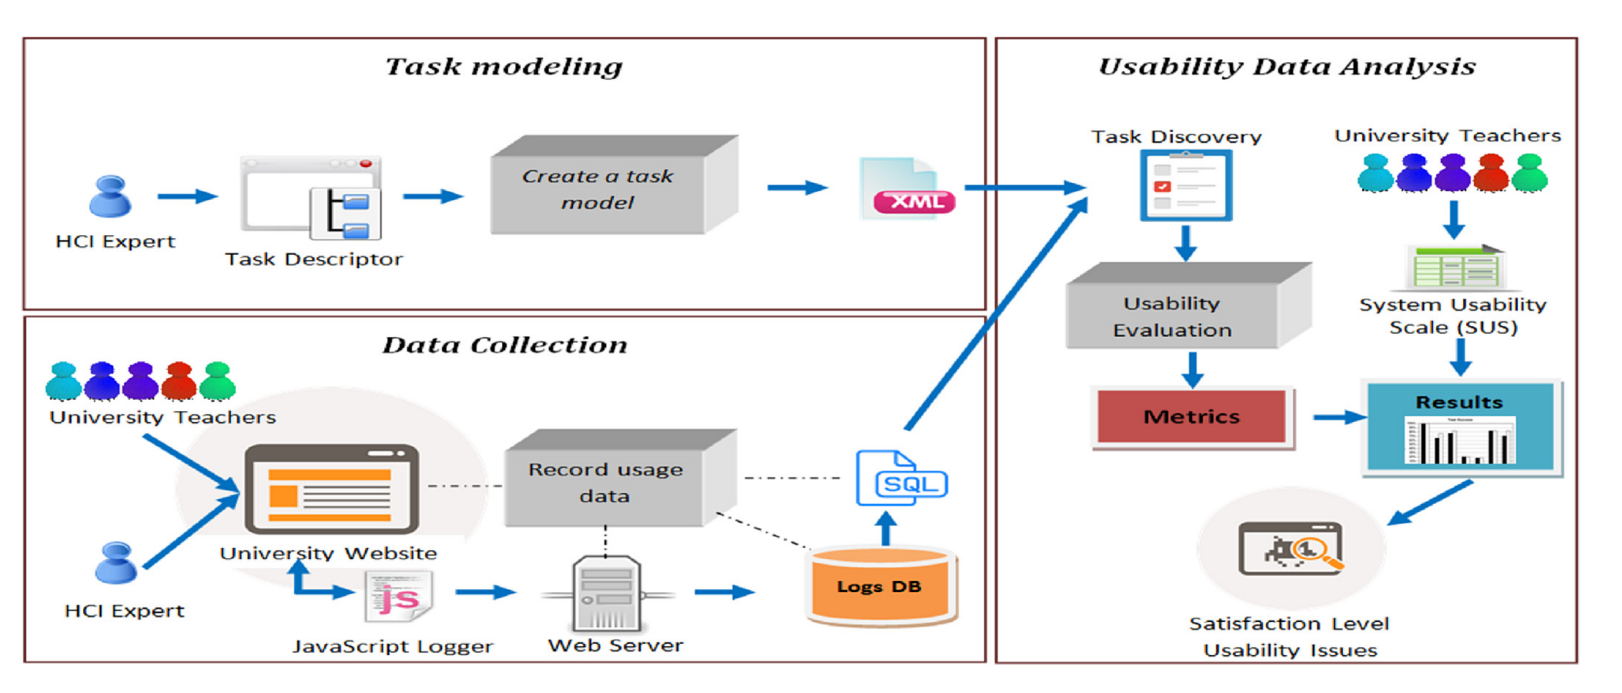
\includegraphics[keepaspectratio=true, width=1\textwidth]{./image/peter.png}
			\caption{\tiny{\cite{harrati2016exploring}}}
		\end{figure}
		
\end{frame}

\section{Zusammenfassung}
\begin{frame}
	\frametitle{Abschluss}
	\begin{columns}
		% Column 1
		\begin{column}{0.5\textwidth}
			\begin{itemize}
				\item <1> Standardisierter Fragebogen
				\item <1> Einfache, schnelle Einschätzung
				\item <1> Kein Vorwissen oder Anleitung für Tester nötig
				\item <1> Nur eine sehr grobe Metrik
			\end{itemize}
		\end{column}
		% Column 2    
		\begin{column}{0.5\textwidth}
			\begin{figure}
				\centering
				
\includegraphics[keepaspectratio=true, width=125px]{./image/sus-meme.png}
				\caption{\tiny{\cite{sp1}}}
			\end{figure}
		\end{column}
	\end{columns}
\end{frame}

\section{Quellen}
\begin{frame}[allowframebreaks, noframenumbering]
    \nocite{*}
	\hfill
	\begin{wrapfigure}{r}{3cm}
		
\includegraphics[keepaspectratio=true, width=100px]{./image/J3Nae.png}
	\end{wrapfigure}
    \bibliographystyle{unsrt}
    \bibliography{references}
\end{frame}

\end{document}